\section{مقدمه}
هدف از این تمرین، طراحی و پیاده‌سازی یک پردازنده‌ی ۳۲ بیتی تک‌چرخه (\lr{Single-Cycle}) به زبان \lr{Verilog} است که توانایی اجرای دستورات محاسباتی، انتقال داده و پرش را داشته باشد. کل پیاده‌سازی در قالب یک فایل واحد و شش ماژول مجزا انجام شده است: ماژول سطح بالا (\lr{\code{main}})، واحد کنترل (\lr{\code{control\_unit}})، بانک ثبات (\lr{\code{regfile}})، واحد حساب و منطق (\lr{\code{alu}}) و دو زیرماژول ترتیبیِ ضرب‌کننده و تقسیم‌کننده (\lr{\code{multiplier}} و \lr{\code{divider}}). تمام بخش‌های پردازنده به‌جز ثبات \lr{\code{PC}}، بانک ثبات و همین دو زیرماژول ضرب/تقسیم کاملاً ترکیبی (\lr{Combinational}) هستند؛ طبق صورت تمرین، عملگرهای ضرب و تقسیم نباید به‌صورت ترکیبی پیاده‌سازی شوند، پس این دو واحد به‌صورت ترتیبی و چندچرخه‌ای ساخته شده‌اند و در طول اجرای خود، پردازنده را موقتاً متوقف می‌کنند.
\section{واحد کنترل (\lr{\code{control\_unit}})}
این ماژول یک مدار ترکیبی است که با دریافت فیلدهای \lr{\code{opcode}} و \lr{\code{funct}} دستور جاری، تمامی سیگنال‌های کنترلی لازم برای هدایت مسیر داده را تولید می‌کند. چون هر دستور دقیقاً در یک چرخه‌ی ساعت کامل اجرا می‌شود، نیازی به جداسازی این واحد به‌صورت یک ماشین حالت سنکرون نبود؛ سیگنال‌ها فقط با یک بلوک \lr{\code{case}} دو سطحی (ابتدا بر اساس \lr{\code{opcode}} و در دستورات \lr{R-type} نیز بر اساس \lr{\code{funct}}) تعیین می‌شوند. سیگنال‌های فعال برای هر دسته از دستورات در جدول زیر آمده است.

\begin{table}[H]
    \centering
    \caption{سیگنال‌های کنترلی فعال برای هر دسته از دستورات}
    \vspace{0.2cm}
    \begin{tabular}{|c|c|p{7.2cm}|}
        \hline
        \textbf{دسته دستور}                & \textbf{نمونه}                                                     & \textbf{سیگنال‌های کنترلی فعال}                                                                                    \\
        \hline
        محاسباتی (\lr{R-type})             & \lr{\code{ADD}}، \lr{\code{SUB}}، \lr{\code{MUL}}، \lr{\code{DIV}} & \lr{\code{RegDst}}=1، \lr{\code{RegWrite}}=1، \lr{\code{ALUControl}} بر اساس \lr{\code{funct}}                    \\
        \hline
        پرش رجیستری (\lr{R-type})          & \lr{\code{JR}}                                                     & \lr{\code{Jr}}=1 (بدون نوشتن در ثبات)                                                                             \\
        \hline
        انتقال داده (\lr{I-type})          & \lr{\code{LW}}، \lr{\code{SW}}                                     & \lr{\code{ALUSrc}}=1، \lr{\code{MemRead}}/\lr{\code{MemWrite}} متناظر، \lr{\code{MemtoReg}}=1 برای \lr{\code{LW}} \\
        \hline
        محاسبه با مقدار ثابت (\lr{I-type}) & \lr{\code{ADDI}}، \lr{\code{SUBI}}، \lr{\code{LUI}}                & \lr{\code{ALUSrc}}=1، \lr{\code{RegWrite}}=1                                                                      \\
        \hline
        پرش شرطی (\lr{I-type})             & \lr{\code{BEQ}}                                                    & \lr{\code{Branch}}=1، \lr{\code{ALUControl}}=\lr{\code{SUB}}                                                      \\
        \hline
        پرش (\lr{J-type})                  & \lr{\code{J}}، \lr{\code{JAL}}                                     & \lr{\code{Jump}}=1، و علاوه‌بر آن \lr{\code{Jal}}=1 و \lr{\code{MemtoReg}}=2 فقط برای \lr{\code{JAL}}              \\
        \hline
    \end{tabular}
\end{table}

علاوه‌بر سیگنال‌های ذکرشده در صورت تمرین، یک سیگنال داخلیِ اضافه به نام \lr{\code{Jr}} هم در این واحد تعریف شده است. دلیلش این است که دستور \lr{\code{JR}}، برخلاف \lr{\code{J}} و \lr{\code{JAL}}، به‌جای استفاده از فیلد آدرس ۲۶ بیتی، مستقیماً مقدار ثبات \lr{\code{rs}} را به \lr{\code{PC}} منتقل می‌کند؛ سیگنال \lr{\code{Jump}} به‌تنهایی برای توصیف این رفتار کافی نبود.

\section{توصیف زیرمدارها}
در این بخش، ساختار و منطق پیاده‌سازی سایر ماژول‌های اصلیِ تشکیل‌دهنده‌ی مسیر داده بررسی می‌شود.

\subsection{ماژول بانک ثبات (\lr{\code{regfile}})}
این ماژول شامل ۳۲ ثبات ۳۲ بیتی با دو درگاه خواندنِ ترکیبی (برای \lr{\code{rs}} و \lr{\code{rt}}) و یک درگاه نوشتنِ سنکرون است. خواندن ثبات \lr{\code{\$0}} مستقل از محتوای حافظه همواره مقدار صفر را بازمی‌گرداند و نوشتن در آن نیز با شرط \lr{\code{WriteReg != 0}} در بلوک نوشتن مسدود می‌شود. از نظر عملکرد، این روش همان کاری را انجام می‌دهد که مالتی‌پلکسر پیشنهادشده در صورت تمرین قرار بود انجام دهد. تمامی ۳۲ ثبات همچنین به‌صورت مستقیم به خروجی‌های ماژول سطح بالا متصل شده‌اند تا وضعیت کامل ثبات‌ها در هر چرخه قابل مشاهده باشد.

\subsection{ماژول حساب و منطق (\lr{\code{alu}}) و واحدهای ترتیبیِ ضرب و تقسیم}
ماژول \lr{\code{alu}} اکنون تنها عملیات جمع، تفریق و شیفت برای \lr{\code{LUI}} را به‌صورت ترکیبی انجام می‌دهد و سیگنال \lr{\code{Zero}} (برای دستور \lr{\code{BEQ}}) را نیز از روی همین خروجی محاسبه می‌کند. طبق صورت تمرین، عملگرهای ترکیبیِ ضرب و تقسیم مجاز نیستند و این دو محاسبه باید به‌صورت ترتیبی پیاده‌سازی شوند؛ به همین دلیل، دو ماژول جداگانه‌ی \lr{\code{multiplier}} و \lr{\code{divider}} دیگر داخل \lr{\code{alu}} نیستند و مستقیماً در \lr{\code{main}} نمونه‌سازی شده‌اند، چون برخلاف \lr{\code{alu}} به سیگنال‌های \lr{\code{Clk}} و \lr{\code{Rst}} نیاز دارند.

هر دو ماژول یک ورودی \lr{\code{Enable}} دارند که از برابریِ \lr{\code{ALUControl}} با کد ضرب یا تقسیم به دست می‌آید. به‌محض فعال‌شدن \lr{\code{Enable}}، عملوندها بارگذاری شده و الگوریتم به‌صورت یک بیت در هر چرخه‌ی ساعت پیش می‌رود: \lr{\code{multiplier}} با روش شیفت-جمع و \lr{\code{divider}} با روش تفریقِ بازگشتیِ بدون‌علامت (\lr{Restoring Division})، با یک رجیستر شیفتیِ ترکیبیِ ۶۴ بیتیِ \lr{\code{\{remainder, quotient\}}}. هر دو محاسبه دقیقاً ۳۲ چرخه طول می‌کشد و در پایان سیگنال \lr{\code{Done}} فعال می‌شود؛ نتیجه و \lr{\code{Done}} تا وقتی \lr{\code{Enable}} غیرفعال نشود (یعنی دستور بعدی \lr{Fetch} شود) ثابت نگه داشته می‌شوند. ماژول ضرب‌کننده در ادامه آمده است:

\begin{latin}
    \begin{lstlisting}[language=Verilog]
module multiplier(
    input  Clk, Rst,
    input  Enable,
    input  [31:0] A, B,
    output reg [31:0] Product,
    output reg Done
);
    reg [31:0] m_cand, m_plier;
    reg [5:0]  count;
    reg        running;

    always @(posedge Clk or posedge Rst) begin
        if (Rst) begin
            running <= 1'b0;
            Done    <= 1'b0;
            Product <= 32'b0;
        end else if (!Enable) begin
            running <= 1'b0;
            Done    <= 1'b0;
        end else if (!running && !Done) begin
            m_cand  <= A;
            m_plier <= B;
            Product <= 32'b0;
            count   <= 6'd0;
            running <= 1'b1;
        end else if (running) begin
            if (m_plier[0])
                Product <= Product + m_cand;
            m_cand  <= m_cand << 1;
            m_plier <= m_plier >> 1;
            if (count == 6'd31) begin
                running <= 1'b0;
                Done    <= 1'b1;
            end else begin
                count <= count + 1;
            end
        end
    end
endmodule
    \end{lstlisting}
\end{latin}

\section{ماژول سطح بالا و مسیر داده (\lr{\code{main}})}
ماژول \lr{\code{main}}، واحد کنترل، بانک ثبات و واحد حساب و منطق را به یکدیگر متصل کرده و ثبات شمارنده‌ی برنامه (\lr{\code{PC}}) را نگه می‌دارد.

طبق جداول قالب دستورات در صورت تمرین (\lr{R-type}، \lr{I-type} و \lr{J-type})، هر فیلد دستور همیشه در یک بازه‌ی بیتیِ ثابت از کلمه‌ی ۳۲ بیتی قرار دارد. به همین دلیل، اولین کار در این ماژول جدا کردن این فیلدها از \lr{\code{InstrIn}} با تکه‌تکه‌کردنِ ترکیبیِ (\lr{Bit-Slicing}) بردار است. تمام این فیلدها بدون توجه به نوع واقعی دستور جاری هم‌زمان استخراج می‌شوند و این واحد کنترل است که بر اساس \lr{\code{opcode}} و \lr{\code{funct}} تشخیص می‌دهد کدام‌یک از آن‌ها برای دستور فعلی معنا دارد. مقدار ۱۶ بیتیِ \lr{\code{imm}} هم با تکرار بیت علامتش (بیت ۱۵) به یک مقدار ۳۲ بیتیِ بسط‌علامت‌دار (\lr{\code{sext\_imm}}) تبدیل می‌شود تا در محاسبات بعدی، مثل آدرس‌دهی \lr{\code{LW}}/\lr{\code{SW}} یا افست \lr{\code{BEQ}}، قابل استفاده باشد:

\begin{latin}
    \begin{lstlisting}[language=Verilog]
wire [5:0]  opcode = InstrIn[31:26];
wire [4:0]  rs     = InstrIn[25:21];
wire [4:0]  rt     = InstrIn[20:16];
wire [4:0]  rd     = InstrIn[15:11];
wire [5:0]  funct  = InstrIn[5:0];
wire [15:0] imm    = InstrIn[15:0];
wire [25:0] jaddr  = InstrIn[25:0];

wire [31:0] sext_imm = {{16{imm[15]}}, imm};
    \end{lstlisting}
\end{latin}

بخش بعدیِ این ماژول، تعیینِ نشانیِ دستوری است که در چرخه‌ی بعد باید واکشی شود. در حالت عادی این مقدار برابر \lr{\code{PC + 4}} است، اما برخی دستورهای صورت تمرین این مقدار پیش‌فرض را تغییر می‌دهند: دستور \lr{\code{JR}} مستقیماً مقدار ثبات \lr{\code{rs}} را جایگزین \lr{\code{PC}} می‌کند، دستورهای \lr{\code{J}} و \lr{\code{JAL}} نشانی را از فیلد ۲۶ بیتیِ آدرس می‌سازند، و دستور \lr{\code{BEQ}} تنها در صورت برابر بودن دو ثبات (یعنی فعال بودن هم‌زمان سیگنال‌های \lr{\code{Branch}} و \lr{\code{Zero}}) به نشانیِ محاسبه‌شده از افست پرش منتقل می‌شود. این بخش از \lr{\code{next\_PC}} با یک مالتی‌پلکسر چهارحالته از میان این گزینه‌ها انتخاب می‌شود؛ اولویت انتخاب نیز دقیقاً به همین ترتیب است: ابتدا \lr{\code{JR}}، سپس \lr{\code{Jump}} (برای \lr{\code{J}}/\lr{\code{JAL}}، با نشانیِ \lr{\code{jump\_target}})، سپس پرش شرطیِ فعال (با نشانیِ \lr{\code{branch\_target}})، و در نهایت در صورت نبودِ هیچ‌کدام، مقدار پیش‌فرضِ \lr{\code{PC + 4}}. چون در هر چرخه حداکثر یکی از این شرایط می‌تواند برقرار باشد، این اولویت‌بندی هیچ‌گاه باعث ابهام در انتخاب نمی‌شود؛ \lr{\code{jump\_target}} و \lr{\code{branch\_target}} نیز دقیقاً مطابق روابط ارائه‌شده در صورت تمرین محاسبه می‌شوند.

از آنجا که طبق صورت تمرین ضرب و تقسیم باید به‌صورت ترتیبی پیاده‌سازی شوند، این دو عملیات دیگر در یک چرخه به پایان نمی‌رسند. برای هماهنگی با این موضوع، یک سیگنال \lr{\code{stall}} در \lr{\code{main}} تعریف شده که تا وقتی دستور جاری \lr{\code{MUL}} یا \lr{\code{DIV}} باشد و سیگنال \lr{\code{Done}}ِ متناظرش هنوز فعال نشده باشد، فعال می‌ماند. تا زمانی که \lr{\code{stall}} فعال است، به‌جای مقدار محاسبه‌شده‌ی بالا، خودِ \lr{\code{PC}} به‌عنوان \lr{\code{next\_PC}} انتخاب می‌شود (یعنی \lr{\code{PC}} ثابت می‌ماند) و سیگنال واقعیِ نوشتن در بانک ثبات نیز با شرط \lr{\code{RegWrite \&\& !stall}} غیرفعال می‌شود تا مقدار ناقصِ میانیِ محاسبه زودتر از موعد در ثبات مقصد نوشته نشود. به‌محض فعال‌شدن \lr{\code{Done}}، \lr{\code{stall}} صفر شده و در همان چرخه هم \lr{\code{PC}} به دستور بعدی می‌رود و هم نتیجه‌ی نهایی در ثبات مقصد نوشته می‌شود. ثبات \lr{\code{PC}} در لبه‌ی بالارونده‌ی ساعت با همین \lr{\code{next\_PC}} به‌روزرسانی می‌شود.

در صورت تمرین ذکر شده که دو بیت کم‌ارزشِ (همواره صفر) نشانی هنگام آدرس‌دهی به حافظه باید نادیده گرفته شوند. از این رو خروجی‌های \lr{\code{InstrAddr}} و \lr{\code{DataAddr}} با شیفت دو بیت به راست نسبت به مقدار داخلیِ \lr{\code{PC}} و خروجی نهاییِ بخش محاسباتی تولید می‌شوند:
\[
    \text{\lr{\code{InstrAddr}}} = \text{\lr{\code{PC}}} \gg 2 \qquad \text{\lr{\code{DataAddr}}} = \text{\lr{\code{final\_result}}} \gg 2
\]
که در آن \lr{\code{final\_result}} بر اساس \lr{\code{ALUControl}}، از میان خروجی \lr{\code{alu}}، \lr{\code{multiplier}} و \lr{\code{divider}} انتخاب می‌شود. البته تمام محاسبات داخلیِ نشانی، مثل آدرس پرش‌های \lr{\code{J}}/\lr{\code{JAL}} و \lr{\code{BEQ}}، بر اساس نشانی بایتی (مضرب ۴) انجام می‌شود و این تبدیل فقط در مرز خروجی به حافظه اعمال می‌شود.

\pagebreak

\section{اجرای آزمون}
برای اطمینان از صحت پردازنده‌ی طراحی‌شده، برنامه‌ی آزمون استاندارد صورت تمرین (شامل محاسبه‌ی دنباله‌ی فیبوناتچی، ضرب دو مقدار و تبدیل حاصل‌ضرب به مبنای سه) با تست‌بنچ رسمی تمرین روی مدار اجرا شد. مقدار هر ثبات در پایان اجرا با مقدار محاسبه‌شده توسط مدار معیار مقایسه شد. خروجی موفقیت‌آمیز اجرای تست‌بنچ در شکل زیر مشاهده می‌شود.

\begin{figure}[H]
    \centering
    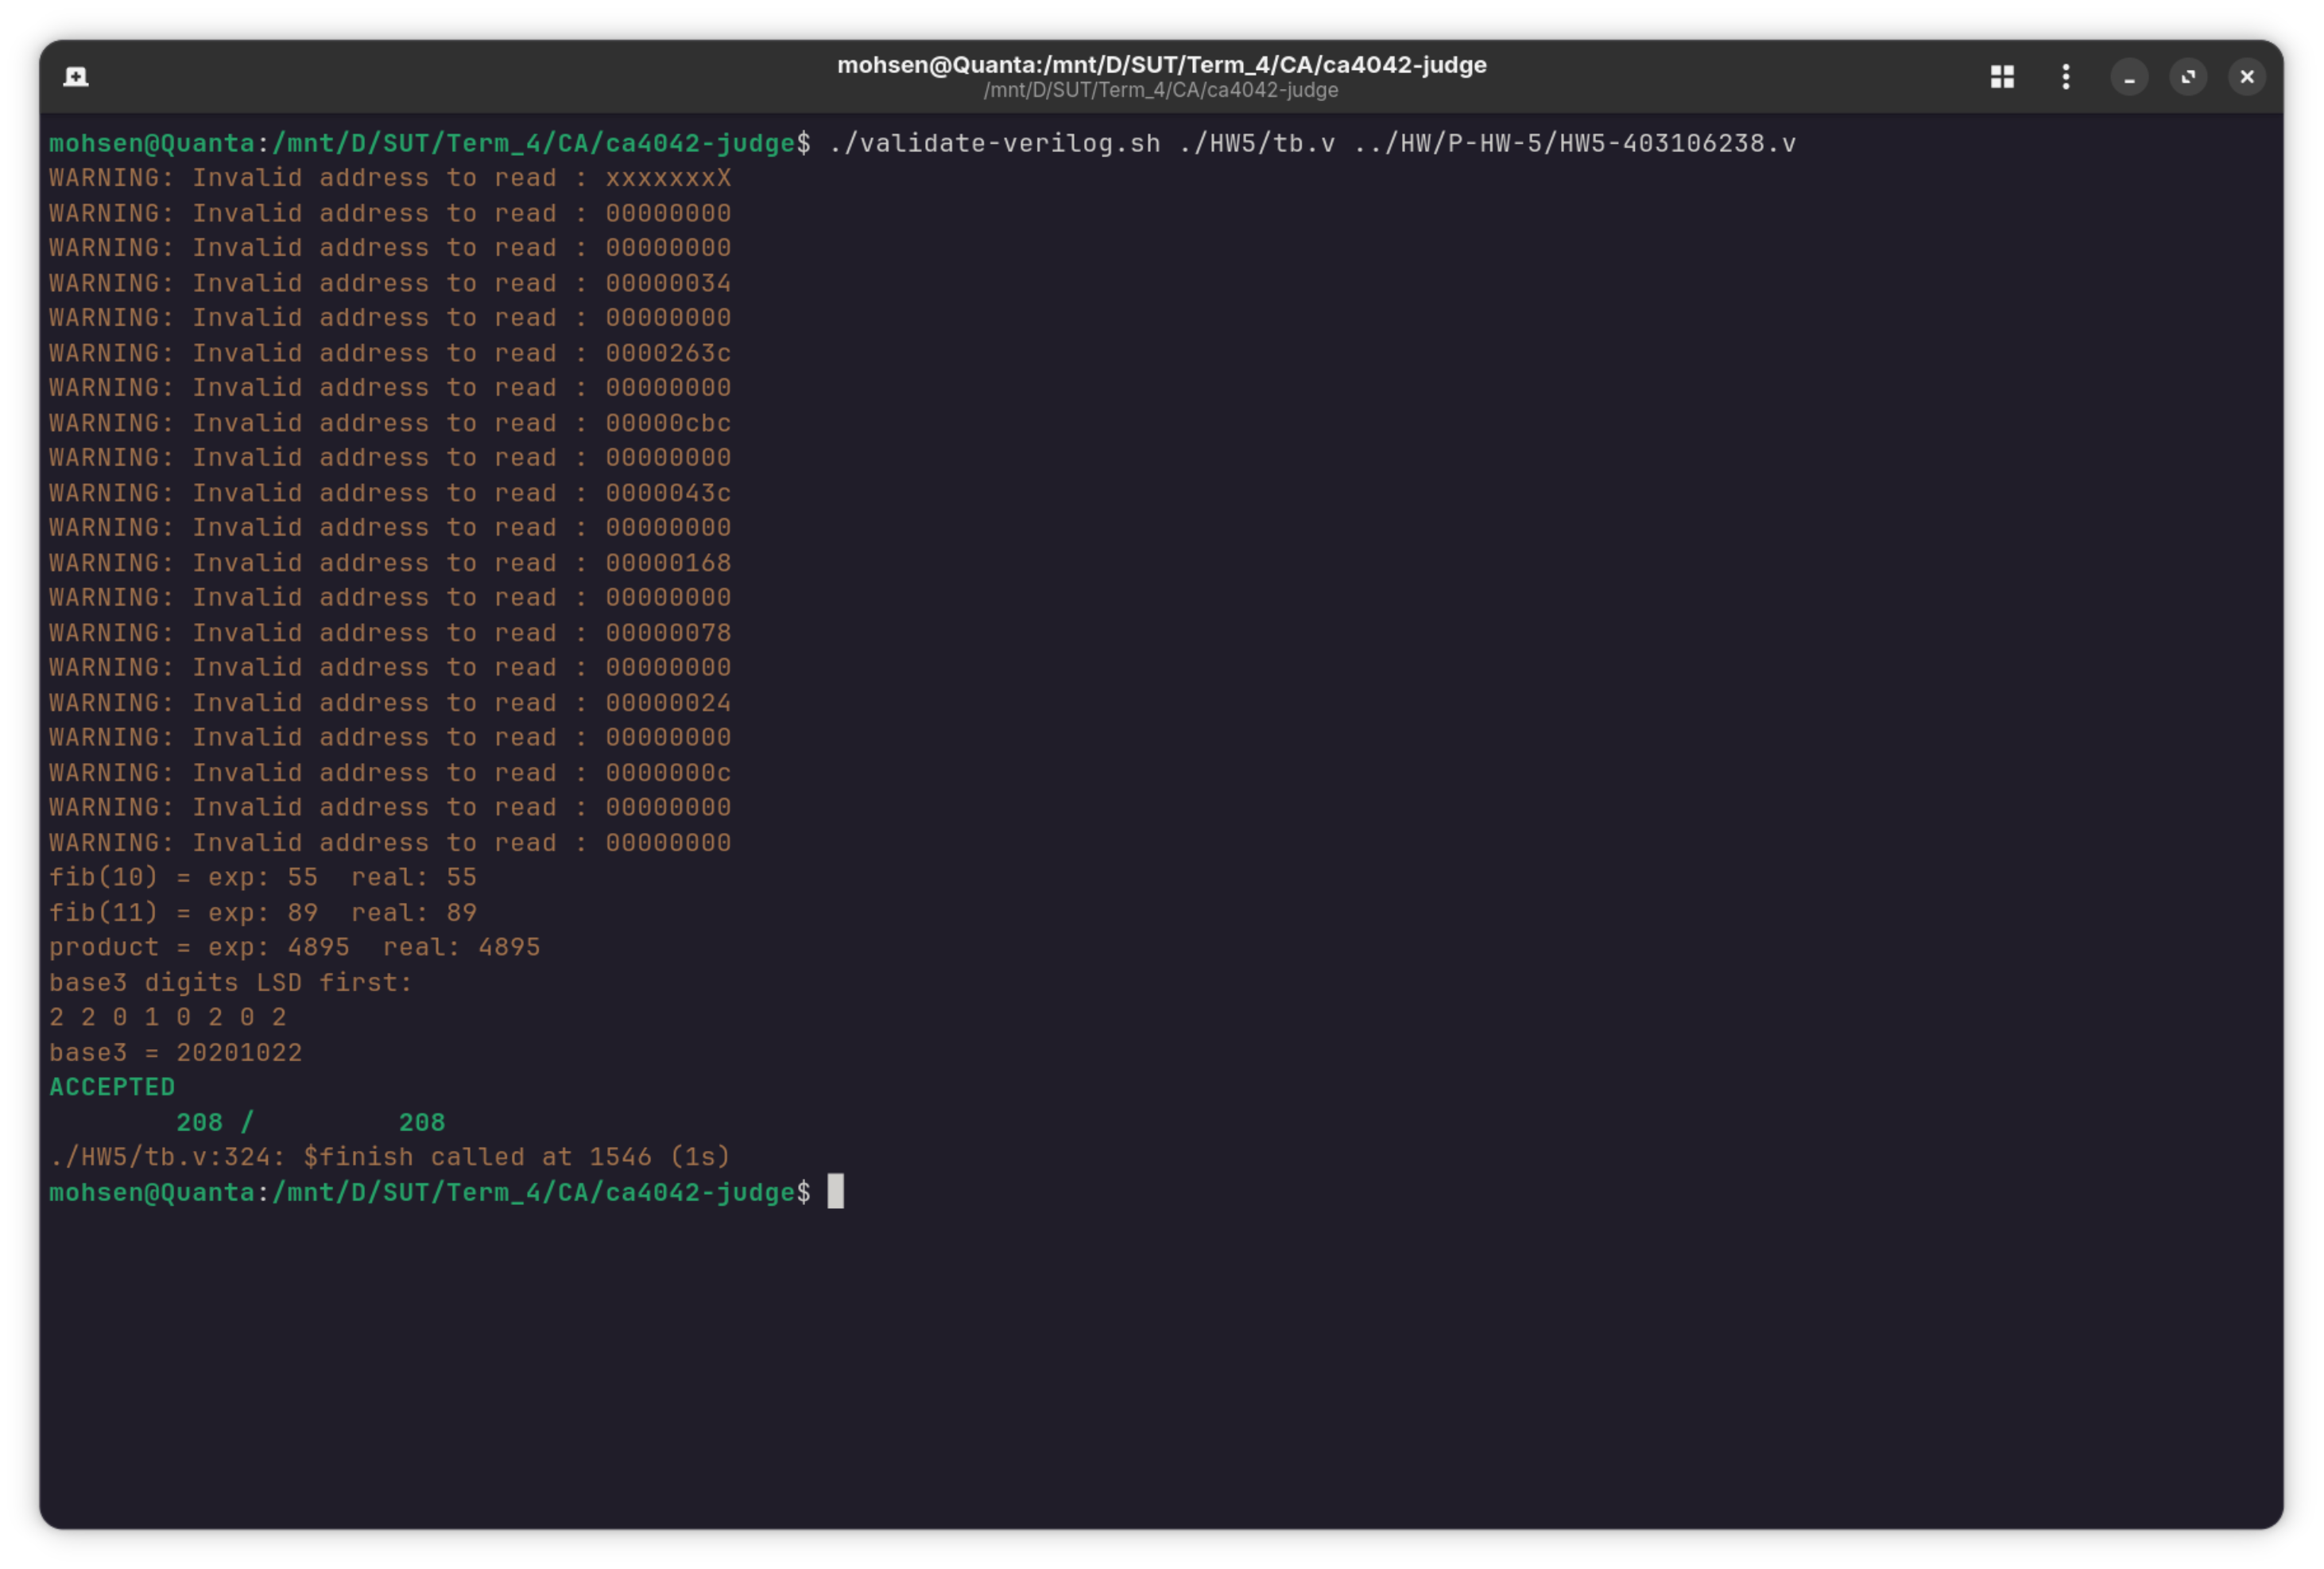
\includegraphics[width=1.0\textwidth]{assets/test_result.png}
    \caption{اجرای تست‌بنچ تمرین}
\end{figure}